\chapter{Nuclear Physics}\label{ch:b3:nuclear-physics}

% Provenance (not for print): first half of the "physique subatomique"
% module common to the surveyed third-year curricula; particle physics
% follows in the next chapter. Deepens the high-school volume's
% radioactivity with SEMF, Gamow tunnelling and reactor physics.

The high-school volume told the story's outline: atoms have nuclei;
some nuclei crumble, on schedules ranging from microseconds to
billions of years; and grams of matter hide megatons of energy. This
chapter reopens the nucleus with Year 3 tools. A droplet model with
five terms predicts the binding of hundreds of \omterm{def:b3:nuclear-physics:nuclide}{nuclides} to the
percent; quantum tunnelling --- the Year 2 volume's barrier problem,
promoted --- explains how one formula spans twenty-five orders of
magnitude in $\alpha$-decay lifetimes; and the binding-energy curve's
quiet maximum at iron divides all of nuclear technology into two
camps: split the heavy (reactors) or join the light (stars, and
someday power plants). The chapter ends beside a reactor pool,
glowing Cherenkov blue.

\section{The nucleus: a saturated drop}

\begin{definition}[Nuclides, size, and density]\label{def:b3:nuclear-physics:nuclide}
\index{nuclide}\index{isotope}\index{nuclear radius}
A \emph{nuclide} $^{A}_{Z}\text{X}$ holds $Z$ protons and $N = A -
Z$ neutrons, bound by the \emph{strong interaction}: intense
(${\sim}\qty{100}{}\times$ Coulomb at contact), short-ranged
(${\sim}\qty{1}{fm}$, felt only by touching neighbours), and blind
to charge (it grips protons and neutrons alike). Scattering
experiments give every nucleus the same recipe: radius
\[
R = r_0A^{1/3} , \qquad r_0 \approx \qty{1.2}{fm} ,
\]
so volume grows like $A$ and the density is a universal
$\rho \approx \qty{2.3e17}{kg/m^3}$ --- a raindrop of it would
weigh like a fleet of tankers, and
\cref{ch:b3:astrophysics} will meet whole stars at this density.
\emph{Isotopes} share $Z$ but differ in $N$: same chemistry,
different nuclear fates.
\end{definition}

\begin{proposition}[Mass defect and binding energy]\label{prop:b3:nuclear-physics:binding}
\index{mass defect}\index{binding energy}\index{iron peak}
A bound nucleus weighs \emph{less} than its parts; by
\cref{ch:b3:relativistic-dynamics}, the missing mass is the
\omterm{prop:b3:nuclear-physics:binding}{binding energy},
\[
B = \big(Zm_{\text{p}} + Nm_{\text{n}} - m_{\text{nucleus}}\big)c^2 ,
\]
typically ${\sim}\qty{8}{MeV}$ \emph{per nucleon} --- a million
times chemistry. Plotted per nucleon, $B/A$ climbs steeply through the light nuclei
(surface effects fade), peaks at $\approx\qty{8.8}{MeV}$ near
iron-56, then drifts down as Coulomb repulsion, long-ranged and
unsaturating, taxes the heavyweights. Both slopes are energy
mines: \emph{fusion} climbs the left slope (the Sun's business),
\emph{fission} rolls down the right (the reactor's) --- and iron,
at the summit, is nuclear ash for both.
\end{proposition}

\begin{omfigure}
\begin{tikzpicture}
  \begin{axis}[omaxis, axis x line=bottom, axis y line=left,
    width=11.2cm, height=6.2cm, xmin=0, xmax=250, ymin=0, ymax=10.3,
    xlabel={mass number $A$}, ylabel={$B/A$ (\unit{MeV})},
    xlabel style={at={(axis description cs:0.5,-0.1)}, anchor=north},
    xtick={56,100,150,200,238}, ytick={2,4,6,8}, clip=false]
    \addplot[omDef, very thick, smooth] coordinates {
      (2,1.11) (3,2.7) (6,5.3) (9,6.46) (12,7.68) (16,7.98)
      (24,8.26) (40,8.55) (56,8.79) (75,8.7) (100,8.6)
      (125,8.45) (150,8.3) (175,8.1) (200,7.9) (220,7.75) (238,7.57)};
    \fill[omThm] (axis cs:4,7.07) circle (1.6pt);
    \draw[gray, thin] (axis cs:12.5,6.85) -- (axis cs:5.2,7.02);
    \node[omThm, font=\scriptsize, anchor=west] at (axis cs:13,6.8)
      {$^4$He};
    \fill[omThm] (axis cs:56,8.79) circle (1.6pt);
    \node[omThm, font=\scriptsize, anchor=south] at (axis cs:56,9.0)
      {$^{56}$Fe: the summit};
    \fill[omThm] (axis cs:238,7.57) circle (1.6pt);
    \node[omThm, font=\scriptsize, anchor=south west] at (axis cs:225,7.85)
      {$^{238}$U};
    \draw[->, omExo, thick] (axis cs:14,4.0) -- (axis cs:40,6.4);
    \node[omExo, font=\scriptsize, anchor=west] at (axis cs:18,3.6)
      {fusion climbs};
    \draw[->, omExo, thick] (axis cs:225,6.4) -- (axis cs:130,7.6);
    \node[omExo, font=\scriptsize, anchor=east] at (axis cs:242,5.9)
      {fission rolls down};
  \end{axis}
\end{tikzpicture}

{\small The binding-energy curve --- arguably the most consequential
graph in physics. Light nuclei gain by merging, heavy ones by
splitting; per kilogram, the left slope pays about four times
better, and the Sun sits on it.}
\end{omfigure}

\begin{proposition}[The semi-empirical mass formula]\label{prop:b3:nuclear-physics:semf}
\index{semi-empirical mass formula}\index{valley of stability}
Model the nucleus as a charged liquid drop and the whole curve
follows from five terms:
\[
B = a_{\text{V}}A - a_{\text{S}}A^{2/3}
- a_{\text{C}}\frac{Z^2}{A^{1/3}}
- a_{\text{A}}\frac{(A - 2Z)^2}{A} + \delta(A) ,
\]
with (in \unit{MeV}) $a_{\text{V}} = 15.8$ (each nucleon bonds its
neighbours: volume), $a_{\text{S}} = 17.8$ (surface nucleons bond
fewer: the drop's ``surface tension''), $a_{\text{C}} = 0.71$
(Coulomb, the long-range saboteur), $a_{\text{A}} = 23.7$
(asymmetry: by \cref{ch:b3:quantum-statistics}, protons and
neutrons fill two separate Fermi ladders, cheapest when equally
full), and $\delta$ a small pairing bonus for even numbers
(\cref{ch:b3:identical-particles}). Minimising at fixed $A$ traces
the \emph{\omterm{prop:b3:nuclear-physics:semf}{valley of stability}}: $N \approx Z$ for light nuclei,
bending neutron-rich ($N/Z \to 1.5$) as Coulomb punishes protons
--- and off-valley \omterm{def:b3:nuclear-physics:nuclide}{nuclides} roll back in by $\beta$ decay.
\end{proposition}
\admitted

\begin{omfigure}
\begin{tikzpicture}
  \begin{axis}[omaxis, axis x line=bottom, axis y line=left,
    width=8.6cm, height=6.4cm, xmin=0, xmax=95, ymin=0, ymax=150,
    xlabel={protons $Z$}, ylabel={neutrons $N$},
    xlabel style={at={(axis description cs:0.5,-0.1)}, anchor=north},
    xtick={20,40,60,80}, ytick={50,100,150}, clip=true]
    \addplot[gray, dashed, domain=0:95] {x};
    \addplot[omDef, very thick, domain=1:92, samples=100]
      {x + 0.03*x^(5/3)};
    \node[gray, font=\scriptsize, anchor=north west] at
      (axis cs:78,74) {$N = Z$};
    \node[omDef, font=\scriptsize, anchor=north west, align=left] at
      (axis cs:48,125) {valley of\\stability};
    \fill (axis cs:26,30) circle (1.5pt);
    \node[font=\scriptsize, anchor=north west] at (axis cs:26,29) {Fe};
    \fill (axis cs:92,146) circle (1.5pt);
    \node[font=\scriptsize, anchor=north west] at (axis cs:88,143) {U};
  \end{axis}
\end{tikzpicture}

{\small The \omterm{prop:b3:nuclear-physics:semf}{valley of stability}. Light nuclei balance their two
Fermi ladders ($N = Z$); heavy ones dilute their Coulomb bill with
extra neutrons. A \omterm{def:b3:nuclear-physics:nuclide}{nuclide} off the valley floor $\beta$-decays back
toward it --- and fission fragments, born far above the line, are
furiously radioactive for exactly this reason.}
\end{omfigure}

\section{Radioactivity, by the clock}

\begin{theorem}[The decay law]\label{thm:b3:nuclear-physics:decay}
\index{radioactive decay law}\index{half-life}\index{activity}
An unstable nucleus has no memory and no aging: in every second it
lives, it decays with the same probability $\lambda$. For $N$
nuclei, $\dd N = -\lambda N\,\dd t$, so
\[
N(t) = N_0\,\eu^{-\lambda t} = N_0\,2^{-t/T_{1/2}} ,
\qquad T_{1/2} = \frac{\ln2}{\lambda} ,
\]
and the \emph{activity} $\mathcal A = \lambda N$ (decays per
second, \unit{Bq}) fades on the same exponential. Half-lives run
from microseconds to billions of years; the statistics of
\cref{ch:b3:microcanonical-ensemble} guarantee that while one
nucleus is perfectly unpredictable, a mole of them keeps
exponential time better than any clock --- the foundation of
radiometric dating.
\end{theorem}

\begin{proof}
Constant per-second probability means $N(t + \dd t) = N(t)(1 -
\lambda\dd t)$; integrate. Setting $N/N_0 = \tfrac12$ gives
$T_{1/2}$.
\end{proof}

\begin{omfigure}
\begin{tikzpicture}
  \begin{axis}[omaxis, axis x line=bottom, axis y line=left,
    width=9.8cm, height=5.6cm, xmin=0, xmax=4.3, ymin=0, ymax=1.12,
    xlabel={$t/T_{1/2}$}, ylabel={$N/N_0$},
    xlabel style={at={(axis description cs:0.5,-0.1)}, anchor=north},
    xtick={1,2,3,4}, ytick={0.25,0.5,1},
    yticklabels={$\tfrac14$,$\tfrac12$,$1$}, clip=true]
    \addplot[omDef, very thick, domain=0:4.3, samples=150]
      {exp(-0.6931*x)};
    \draw[gray, dashed] (axis cs:0,0.5) -| (axis cs:1,0);
    \draw[gray, dashed] (axis cs:0,0.25) -| (axis cs:2,0);
    \node[font=\scriptsize, anchor=south west, align=left] at
      (axis cs:2.3,0.55) {each half-life\\halves the count};
  \end{axis}
\end{tikzpicture}

{\small Exponential decay: memoryless individuals, punctual
population. Two half-lives leave a quarter; ten leave a
thousandth --- the ruler with which physicists date charcoal,
glaciers, and the Earth.}
\end{omfigure}

\begin{remark}[Three doors out of a nucleus]\label{rem:b3:nuclear-physics:modes}
\index{alpha decay}\index{beta decay}\index{gamma decay}\index{Gamow model}
$\boldsymbol\alpha$: a heavy nucleus emits a $^4$He cluster. Classically
impossible --- the Coulomb barrier tops \qty{25}{MeV} and the
$\alpha$ leaves with \qty{5}{}--\qty{9}{MeV} --- it happens by
\emph{tunnelling} (the Year 2 volume's barrier, curved): Gamow's
exponential sensitivity turns a factor two in energy into twenty
orders of magnitude in lifetime, exactly the Geiger--Nuttall
pattern (\cref{exo:b3:nuclear-physics:8}).
$\boldsymbol\beta$: a neutron becomes a proton (or vice versa), emitting
an electron (or positron) and a neutrino --- the \emph{weak
interaction} at work, the valley-restoring force; the neutrino's
story waits for \cref{ch:b3:particle-physics}.
$\boldsymbol\gamma$: an excited nucleus sheds \unit{MeV} photons, the
nuclear analogue of \cref{ch:b3:hydrogen-atom}'s spectral lines.
Decays chain until the valley floor is reached: uranium's ladder
ends, fourteen rungs later, at stable lead.
\end{remark}

\section{Down the slopes: fission and fusion}

\begin{proposition}[Fission and the chain reaction]\label{prop:b3:nuclear-physics:fission}
\index{fission}\index{chain reaction}\index{critical mass}
A slow neutron absorbed by $^{235}$U makes a wobbling drop that
splits: two mid-mass fragments, two-to-three fresh neutrons, and
$\approx\qty{200}{MeV}$ --- the $B/A$ gap between uranium's
\qty{7.6}{MeV} and the fragments' \qty{8.5}{MeV}, times 235.
The freed neutrons can fission further nuclei: with
multiplication factor $k$ (neutrons per neutron, one generation
later), a population grows as $k^n$ --- subcritical ($k < 1$)
dies out, critical ($k = 1$) holds steady, supercritical explodes.
A reactor moderates neutrons to slow speeds (fission's preferred
diet), leans on the 0.7\,\% of neutrons that arrive
\emph{seconds} late from fragment decays --- the delay that makes
$k \approx 1$ humanly adjustable --- and lets control rods eat
the surplus (\cref{pb:b3:nuclear-physics:1}).
\end{proposition}
\admitted

\begin{omfigure}
\begin{tikzpicture}[scale=1.0]
  % stage 1: nucleus + neutron
  \draw[->, thick] (-1.3,0) -- (-0.55,0);
  \fill[gray] (-1.55,0) circle (2.6pt);
  \node[font=\scriptsize, anchor=south] at (-1.55,0.12) {n};
  \draw[omDef, fill=omDef!15, thick] (0.35,0) circle (0.62);
  \node[omDef, font=\scriptsize] at (0.35,0) {$^{235}$U};
  % arrow
  \draw[->, thick] (1.35,0) -- (2.05,0);
  % stage 2: deformed drop (peanut)
  \draw[omDef, fill=omDef!15, thick, rotate around={0:(3.1,0)}]
    (3.1,0) ellipse (0.85 and 0.42);
  \draw[omDef!60, dashed] (3.1,-0.5) -- (3.1,0.5);
  % arrow
  \draw[->, thick] (4.3,0) -- (5.0,0);
  % stage 3: fragments + neutrons
  \draw[omThm, fill=omThm!12, thick] (5.9,0.55) circle (0.42);
  \draw[omThm, fill=omThm!12, thick] (5.9,-0.55) circle (0.42);
  \node[omThm, font=\tiny] at (5.9,0.55) {Ba};
  \node[omThm, font=\tiny] at (5.9,-0.55) {Kr};
  \foreach \ang in {15,-8,40}{
    \fill[gray] ({6.7+0.35*cos(\ang)},{0.3*sin(\ang)}) circle (2.2pt);
    \draw[->, gray] ({6.95+0.35*cos(\ang)},{0.32*sin(\ang)}) --
      ({7.55+0.35*cos(\ang)},{0.42*sin(\ang)});}
  \node[font=\scriptsize, anchor=west, align=left] at (8.05,0)
    {2--3 neutrons\\$+\ \qty{200}{MeV}$};
\end{tikzpicture}

{\small Liquid-drop fission: a slow neutron sets $^{235}$U
wobbling; the deformed drop's Coulomb repulsion beats its surface
tension, and it tears into neutron-rich fragments plus the spare
neutrons that make a chain possible.}
\end{omfigure}

\begin{remark}[Fusion: the harder, better slope]\label{rem:b3:nuclear-physics:fusion}
\index{fusion}
Joining light nuclei pays $\sim4\times$ more per kilogram than
splitting heavy ones, with no long-lived fragments --- but the
reactants, both positive, must tunnel through their mutual Coulomb
barrier, which demands temperatures of $10^7$--$10^8\,\unit{K}$
(\cref{exo:b3:nuclear-physics:11}). Stars do it by being enormous
(\cref{ch:b3:astrophysics}: the Sun turns \qty{600}{} million
tonnes of hydrogen into helium each second); laboratories do it
with magnetically bottled plasmas and, so far, an energy ledger
still shy of its break-even ambitions.
\end{remark}

\begin{omfigure}
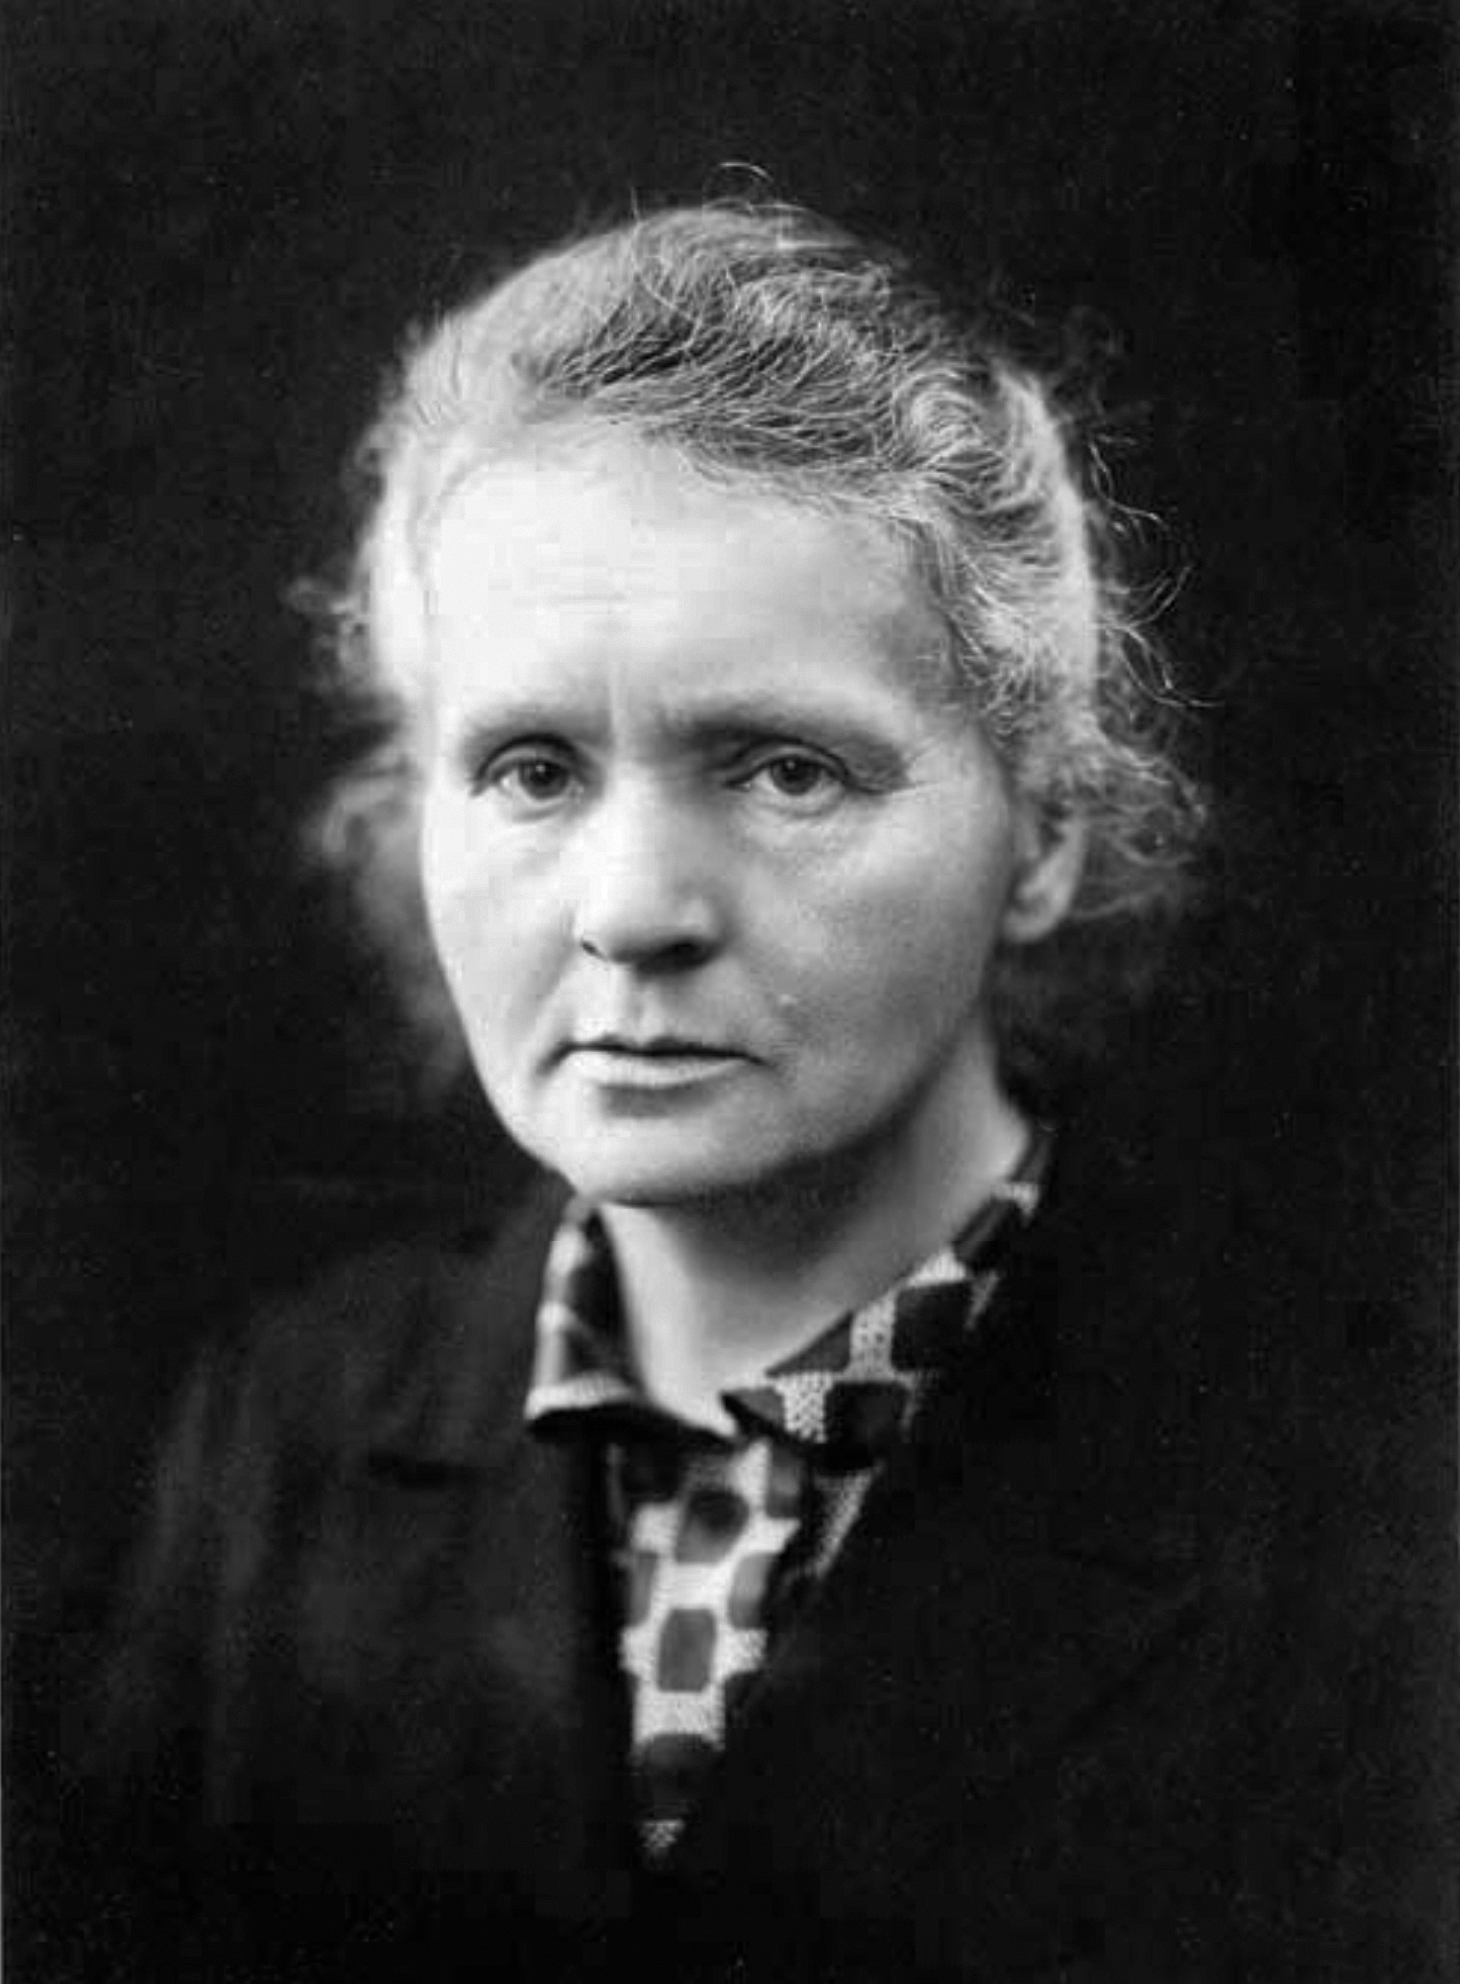
\includegraphics[width=0.34\linewidth]{images/book5/photo-marie-curie.jpg}

{\small Marie Curie (photograph by Henri Manuel, c.~1920, public domain): twice a Nobel laureate for opening this chapter's subject --- the gram of radium of \cref{exo:b3:nuclear-physics:4} was hers.}
\end{omfigure}

\section{Exercises}

\begin{exercise}[$\star$]\label{exo:b3:nuclear-physics:1}
Bookkeeping. (a) Give $Z$, $N$, $A$ for $^{12}$C, $^{14}$C,
$^{235}$U, $^{238}$U. (b) Which pairs are \omterm{def:b3:nuclear-physics:nuclide}{isotopes}? (c) Why do
\omterm{def:b3:nuclear-physics:nuclide}{isotopes} share chemistry but not nuclear stability? (d) $^{14}$C
and $^{14}$N share $A = 14$: what are such \omterm{def:b3:nuclear-physics:nuclide}{nuclides} called, and
what decay connects them?
\end{exercise}

\begin{exercise}[$\star$]\label{exo:b3:nuclear-physics:2}
The universal density. (a) From $R = r_0A^{1/3}$, show the
nuclear density is independent of $A$ and evaluate it. (b)
Compute the mass of a teaspoon (\qty{5}{mL}) of nuclear matter.
(c) What fraction of an atom's volume does its nucleus fill (take
$R_{\text{atom}} = \qty{1e-10}{m}$, $A = 60$)? (d) What does the
$A^{1/3}$ law itself say about the strong force's range?
\end{exercise}

\begin{exercise}[$\star$]\label{exo:b3:nuclear-physics:3}
Weighing the glue. Nuclear masses: $m_{\text{p}} =
\qty{1.007276}{u}$, $m_{\text{n}} = \qty{1.008665}{u}$,
$m(^4\text{He}) = \qty{4.001506}{u}$;
$\qty{1}{u}\,c^2 = \qty{931.5}{MeV}$. (a) Compute $^4$He's \omterm{thm:b3:relativistic-dynamics:emc2}{mass
defect} and \omterm{prop:b3:nuclear-physics:binding}{binding energy}. (b) Give $B/A$. (c) Compare $B$ with
the \qty{13.6}{eV} of \cref{ch:b3:hydrogen-atom}: how many orders
of magnitude separate nuclear from atomic glue? (d) Why does
$^4$He's exceptional binding (the figure's spike) make it the
currency of $\alpha$ decay?
\end{exercise}

\begin{exercise}[$\star$]\label{exo:b3:nuclear-physics:4}
The first curie. Radium-226: $T_{1/2} = 1600$ years, molar mass
\qty{226}{g/mol}. For one gram: (a) count the nuclei; (b) compute
$\lambda$; (c) compute the activity and compare with the historic
unit $1\,\text{Ci} = \qty{3.7e10}{Bq}$ (defined as exactly this
gram); (d) how much of the gram survives after 4800 years?
\end{exercise}

\begin{exercise}[$\star\star$]\label{exo:b3:nuclear-physics:5}
The formula at work. With $a_{\text{V}} = 15.75$,
$a_{\text{S}} = 17.8$, $a_{\text{C}} = 0.711$,
$a_{\text{A}} = 23.7$ (\unit{MeV}) and pairing
$+12/\sqrt A$ for even--even nuclei: (a) compute the four main
terms of $B$ for $^{56}$Fe ($Z = 26$). (b) Sum (with pairing) and
compare $B/A$ with the measured \qty{8.79}{MeV}. (c) Which two
terms fight hardest, and what does their balance set? (d) Why
must the Coulomb term, alone, grow \emph{faster} than $A$?
\end{exercise}

\begin{exercise}[$\star\star$]\label{exo:b3:nuclear-physics:6}
The valley floor. (a) Keeping only the $Z$-dependent terms,
minimise the mass at fixed $A$ and derive
$Z^* = \dfrac{A/2}{1 + a_{\text{C}}A^{2/3}/4a_{\text{A}}}$. (b)
Evaluate for $A = 101$ and compare with ruthenium ($Z = 44$).
(c) Show the light-$A$ limit is $Z^* = A/2$ and interpret with
the two Fermi ladders. (d) A fission fragment has $A = 95$,
$Z = 36$: how far off the valley is it, and what sequence of
decays follows?
\end{exercise}

\begin{exercise}[$\star\star$]\label{exo:b3:nuclear-physics:7}
Radiocarbon. Living matter keeps $^{14}$C
($T_{1/2} = 5730$ years) topped up at 1 atom per $10^{12}$
carbons; death stops the refill. (a) A charcoal sample shows
30\,\% of the living activity: how old is the fire? (b) One gram
of living carbon: compute its $^{14}$C activity
($\approx\qty{0.23}{Bq}$ expected). (c) Why is the method useless
beyond $\sim\qty{50000}{}$ years? (d) And why is it useless for
dating rocks (which clocks take over)?
\end{exercise}

\begin{exercise}[$\star\star$]\label{exo:b3:nuclear-physics:8}
Gamow's cliff. Polonium-212 emits an \qty{8.78}{MeV} $\alpha$;
its barrier tops $\approx\qty{26}{MeV}$. (a) Show classical
escape is impossible, and classical entry too --- yet it decays
in \qty{0.3}{\micro s}. (b) Uranium-238's $\alpha$ carries
\qty{4.2}{MeV} and its half-life is $4.5\times10^9$ years:
compute the ratio of the two decay constants. (c) Explain, with
the tunnelling exponential, how a factor two in energy buys
$\sim10^{24}$ in rate. (d) Why does the same physics set the
Sun's core temperature requirement?
\end{exercise}

\begin{exercise}[$\star\star$]\label{exo:b3:nuclear-physics:9}
Two hundred million electron-volts. (a) Justify the
$\qty{200}{MeV}$ per fission from the $B/A$ curve. (b) Compute
the energy in one kilogram of $^{235}$U fully fissioned, in
joules and in tonnes of oil equivalent
(\qty{42}{GJ/t}). (c) A \qty{1}{GW_e} power plant at 33\,\%
efficiency: how many kilograms of $^{235}$U per year? (d) Why do
the fragments, not the neutrons, carry most of the
\qty{200}{MeV}, and into what form does it immediately go?
\end{exercise}

\begin{exercise}[$\star\star\star$]\label{exo:b3:nuclear-physics:10}
Taming $k$. In a reactor, prompt neutrons reproduce in $\ell
\approx \qty{e-4}{s}$. (a) With $k = 1.001$ on prompt neutrons
alone, compute the power multiplication in one second --- and the
verdict on mechanical control. (b) A fraction $\beta =
0.7\,\%$ of neutrons is \emph{delayed} by $\sim\qty{10}{s}$:
explain why, for $k - 1 < \beta$, the chain's effective clock
becomes seconds. (c) Compute the same one-second multiplication
with the effective generation time $\sim\qty{0.1}{s}$. (d) State
in one sentence what Chernobyl's operators lost when their
reactor went prompt-supercritical.
\end{exercise}

\begin{exercise}[$\star\star\star$]\label{exo:b3:nuclear-physics:11}
The Sun's arithmetic. Overall, $4\,^1\text{H} \to {}^4\text{He}$
converts \qty{0.71}{\percent} of the mass to energy
(\qty{26.7}{MeV}, neutrinos included). (a) From $L_\odot =
\qty{3.8e26}{W}$, compute the mass converted per second, and the
hydrogen consumed per second. (b) With $\qty{2e30}{kg}$ of sun,
a tenth of it burnable core hydrogen (take the hydrogen fraction
$\approx0.75$): estimate the lifetime. (c) Two protons at
\qty{1.5e7}{K}: compare $k_{\text{B}}T$ with their Coulomb
barrier at \qty{1}{fm} and conclude who does the crossing
(\cref{exo:b3:nuclear-physics:8}). (d) Why does fusion, unlike
fission, leave essentially no radioactive ash?
\end{exercise}

\begin{exercise}[$\star\star\star$]\label{exo:b3:nuclear-physics:12}
Nuclear medicine. (a) Technetium-99m ($T_{1/2} = \qty{6}{h}$,
$\gamma$ of \qty{140}{keV}) is medicine's workhorse: compute the
number of nuclei, and their mass, behind an injected
\qty{500}{MBq}. (b) Explain why a six-\emph{hour} half-life and a
pure $\gamma$ are each exactly what a diagnostic wants. (c) PET:
a positron from $^{18}$F annihilates with an electron ---
use \cref{ch:b3:relativistic-dynamics} to give the energy and
geometry of the two photons, and hence the detector's principle.
(d) Radiotherapy delivers \qty{2}{Gy} (\unit{J/kg}) to a tumour:
compare the energy with a sip of warm water, and reconcile the
harmlessness of the joules with the lethality of the ionisation.
\end{exercise}

\begin{omfigure}
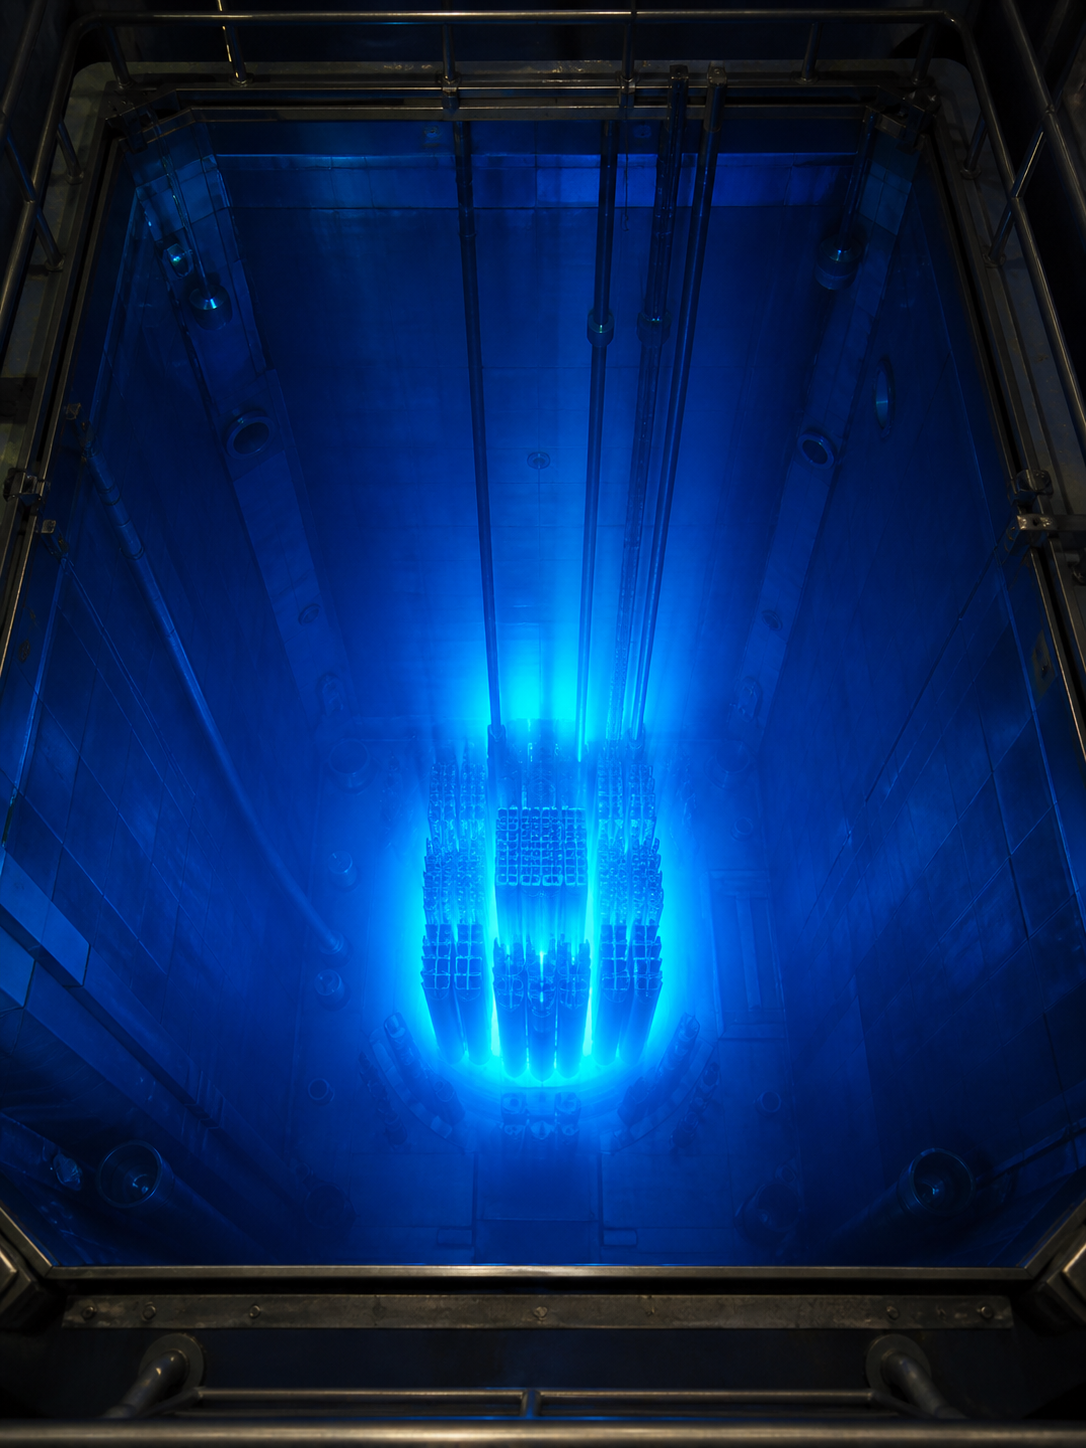
\includegraphics[width=0.45\linewidth]{images/book5/ai/b5-21-cherenkov-pool.png}

{\small The reactor pool of the weekend problem: fragment $\beta$ electrons outrunning light in water wrap the core in Cherenkov blue --- the shielding, visibly at work.}
\end{omfigure}

\section{Problem: Open day at the research reactor}

\begin{problem}\label{pb:b3:nuclear-physics:1}
\emph{Open day at the research reactor.} The national laboratory
opens its \qty{20}{MW} pool-type research reactor to visitors, and
you have talked your way onto the balcony: below, through eight
metres of limpid water, the core glows an unearthly blue. The
guide --- a retiring reactor physicist --- has agreed to let you
do the arithmetic.

\medskip\noindent\textbf{Part I --- The energy ledger.}

\begin{enumerate}
  \item Each fission of $^{235}$U releases about \qty{200}{MeV}.
        Convert to joules, and compute the fissions per second
        sustaining \qty{20}{MW}.
  \item Convert to grams of $^{235}$U consumed per day.
  \item The same \qty{20}{MW} from coal (\qty{30}{MJ/kg}): tonnes
        per day? Form the mass ratio and connect it to the
        \qty{}{MeV}-versus-\qty{}{eV} scales of this chapter and
        chemistry.
  \item The fragments are born at $\sim\qty{8.5}{MeV}$ per
        nucleon binding, uranium at \qty{7.6}{MeV}: verify
        $235\times0.9 \approx \qty{200}{MeV}$ is consistent.
  \item The fragments stop within micrometres of their birthplace.
        Into what does their \qty{200}{MeV} convert, and on what
        timescale does it reach the cooling water?
  \item Why are the fragments (e.g.\ $A = 95$, $Z = 36$)
        inevitably radioactive? Use the \omterm{prop:b3:nuclear-physics:semf}{valley of stability}.
\end{enumerate}

\medskip\noindent\textbf{Part II --- Keeping $k = 1$.}

\begin{enumerate}[resume]
  \item Define the multiplication factor $k$ and state what
        $k = 0.999$, $1.000$, $1.001$ mean for the neutron
        population.
  \item The pool water moderates. Explain in two sentences why
        slowing neutrons to thermal speeds \emph{helps} fission
        $^{235}$U, and why hydrogen is the best moderator
        (recall elastic collisions from the Year 1 volume).
  \item Control rods are boron steel. What does boron do, and
        how does raising or lowering the rods steer $k$?
  \item With prompt neutrons alone ($\ell = \qty{e-4}{s}$) and
        $k = 1.0005$, compute the power growth over one second
        and conclude.
  \item The 0.7\,\% delayed neutrons stretch the effective
        generation time to $\sim\qty{0.1}{s}$: recompute, and
        state the design rule that keeps $k - 1$ safely below
        the delayed fraction.
  \item The water is also the coolant. Explain the intrinsic
        safety feature: what happens to moderation --- and hence
        to $k$ --- if the water boils away?
  \item Why does the reactor still need emergency cooling after
        shutdown? (Name the heat source that control rods cannot
        touch.)
\end{enumerate}

\medskip\noindent\textbf{Part III --- The blue light.}

\begin{enumerate}[resume]
  \item The glow is Cherenkov radiation: light's speed in water
        is $c/n$ with $n = 1.33$. What must a charged particle do
        to emit it?
  \item Compute the threshold speed, and with
        \cref{ch:b3:relativistic-dynamics} the threshold kinetic
        energy for an electron.
  \item Which reactor particles qualify? Trace the chain from
        fission fragment to fast $\beta$ electron in the water.
  \item The spectrum's intensity grows toward short wavelengths:
        why does the pool glow blue rather than red?
  \item The guide says: ``the glow \emph{is} the shielding
        working.'' Explain --- what does eight metres of water do
        to the core's radiation, and roughly why is the balcony
        safe?
  \item After shutdown the blue dims over minutes but does not
        vanish for days. Connect to Part I's question 6.
\end{enumerate}

\medskip\noindent\textbf{Part IV --- What the reactor is for.}

\begin{enumerate}[resume]
  \item This reactor's day job is making molybdenum-99
        ($T_{1/2} = \qty{66}{h}$), parent of medicine's
        technetium-99m. Why must the world's hospitals be
        resupplied weekly, and why can no warehouse stockpile it?
  \item A \qty{100}{GBq} Mo-99 shipment leaves on Monday; the
        hospital elutes Tc-99m on Friday (96 hours later). What
        activity of the parent remains?
  \item Neutron beams from the core also feed the diffraction
        instruments of \cref{ch:b3:crystalline-solids}: why are
        reactor neutrons, once thermalised, born with the right
        wavelength?
  \item The guide's parting problem: a fuel element spends five
        years in the pool before shipment. Using the fragments'
        mix of half-lives, explain the logic --- what has five
        years of pool time bought?
  \item Estimate the decay heat one hour after shutdown
        ($\approx1\,\%$ of \qty{20}{MW}) and compare it with a
        household's electric heater: is passive pool cooling
        plausible?
  \item Close the ledger in four lines: $B/A$ pays
        \qty{200}{MeV} a split; delayed neutrons lend the
        seconds that make $k$ steerable; water moderates,
        cools, shields, and glows; and the day's real product
        leaves in medical vials, not megawatts.
\end{enumerate}
\end{problem}
